\section{Příklad 5}
\sloppy
% Jako parametr zadejte skupinu (A-H)
\patyZadani{F}

\subsection*{Z ceho budeme vychaze}
\[
i = \frac{U_r}{R} \quad \Rightarrow \quad \text{Ohmův zákon}
\]

\[
U_r + U_r = U \quad \Rightarrow \quad \text{Kirchhoffův druhý zákon}
\]

\[
i' = \frac{U_c}{L}, \quad i(0) = i_{L_0}
\]
\subsection*{Samotny vypocet}
\textbf{Kroky:}
1. Nejprve vyjádříme \( U_r \) z první rovnice.
2. Dosadíme \( U_r \) do druhé rovnice.
3. Poté dosadíme výsledek do třetí rovnice.

\[
i' = \frac{U}{L} - \frac{R}{L} \times i
\]

\textbf{Úprava:}

\[
L \times i' + R \times i = U
\]

\textbf{Charakteristická rovnice:}

\[
L\lambda + R = 0 \quad \Rightarrow \quad \lambda = \frac{-R}{L}
\]

\textbf{Očekávané řešení:}

\[
i(t) = I_L e^{\lambda t} \quad \Rightarrow \quad I_L(t) = I_L e^{\frac{-R}{L} t}
\]

\textbf{Dosadíme do upravené rovnice:}

\[
I_L'(t) = \frac{U}{L} e^{\frac{R}{L} t}
\]

\textbf{Jelikož se jedná o derivaci, musíme integrovat:}

\[
\frac{U}{L} \int e^{\frac{R}{L} t} \, dt
\]


\textbf{Substituce:} \( u = \frac{R}{L} t \quad \Rightarrow \quad du = \frac{R}{L} \, dt \)

\[
\frac{du}{dt} = \frac{R}{L}, \quad \text{takže} \quad dt = \frac{L}{R} du
\]

\[
\frac{U}{L} \int e^u \times \frac{L}{R} \, du
\]

\textbf{Zjednodušení:}

\[
\frac{U}{L} \times \frac{L}{R} \int e^u \, du
\]

\[
\frac{U}{R} e^u + C
\]


\textbf{Dosadíme zpět:}

\[
I_l = \frac{U}{R} + i(0) \cdot e^{\frac{R}{L} \cdot t}
\]
\[
    i(0) = _{LP} \rightarrow 8 - \frac{U}{R} = i(0)
\]

\[
    I_L = \frac{U}{R} + (8 - \frac{U}{R}) \times e^{\frac{R}{L} t}
\]
\[
I_L = \frac{1}{2} + \frac{15}{2} \times e^ {-5 \times t}
\]
graf prubehu:

\begin{figure}[!ht]
  \centering
  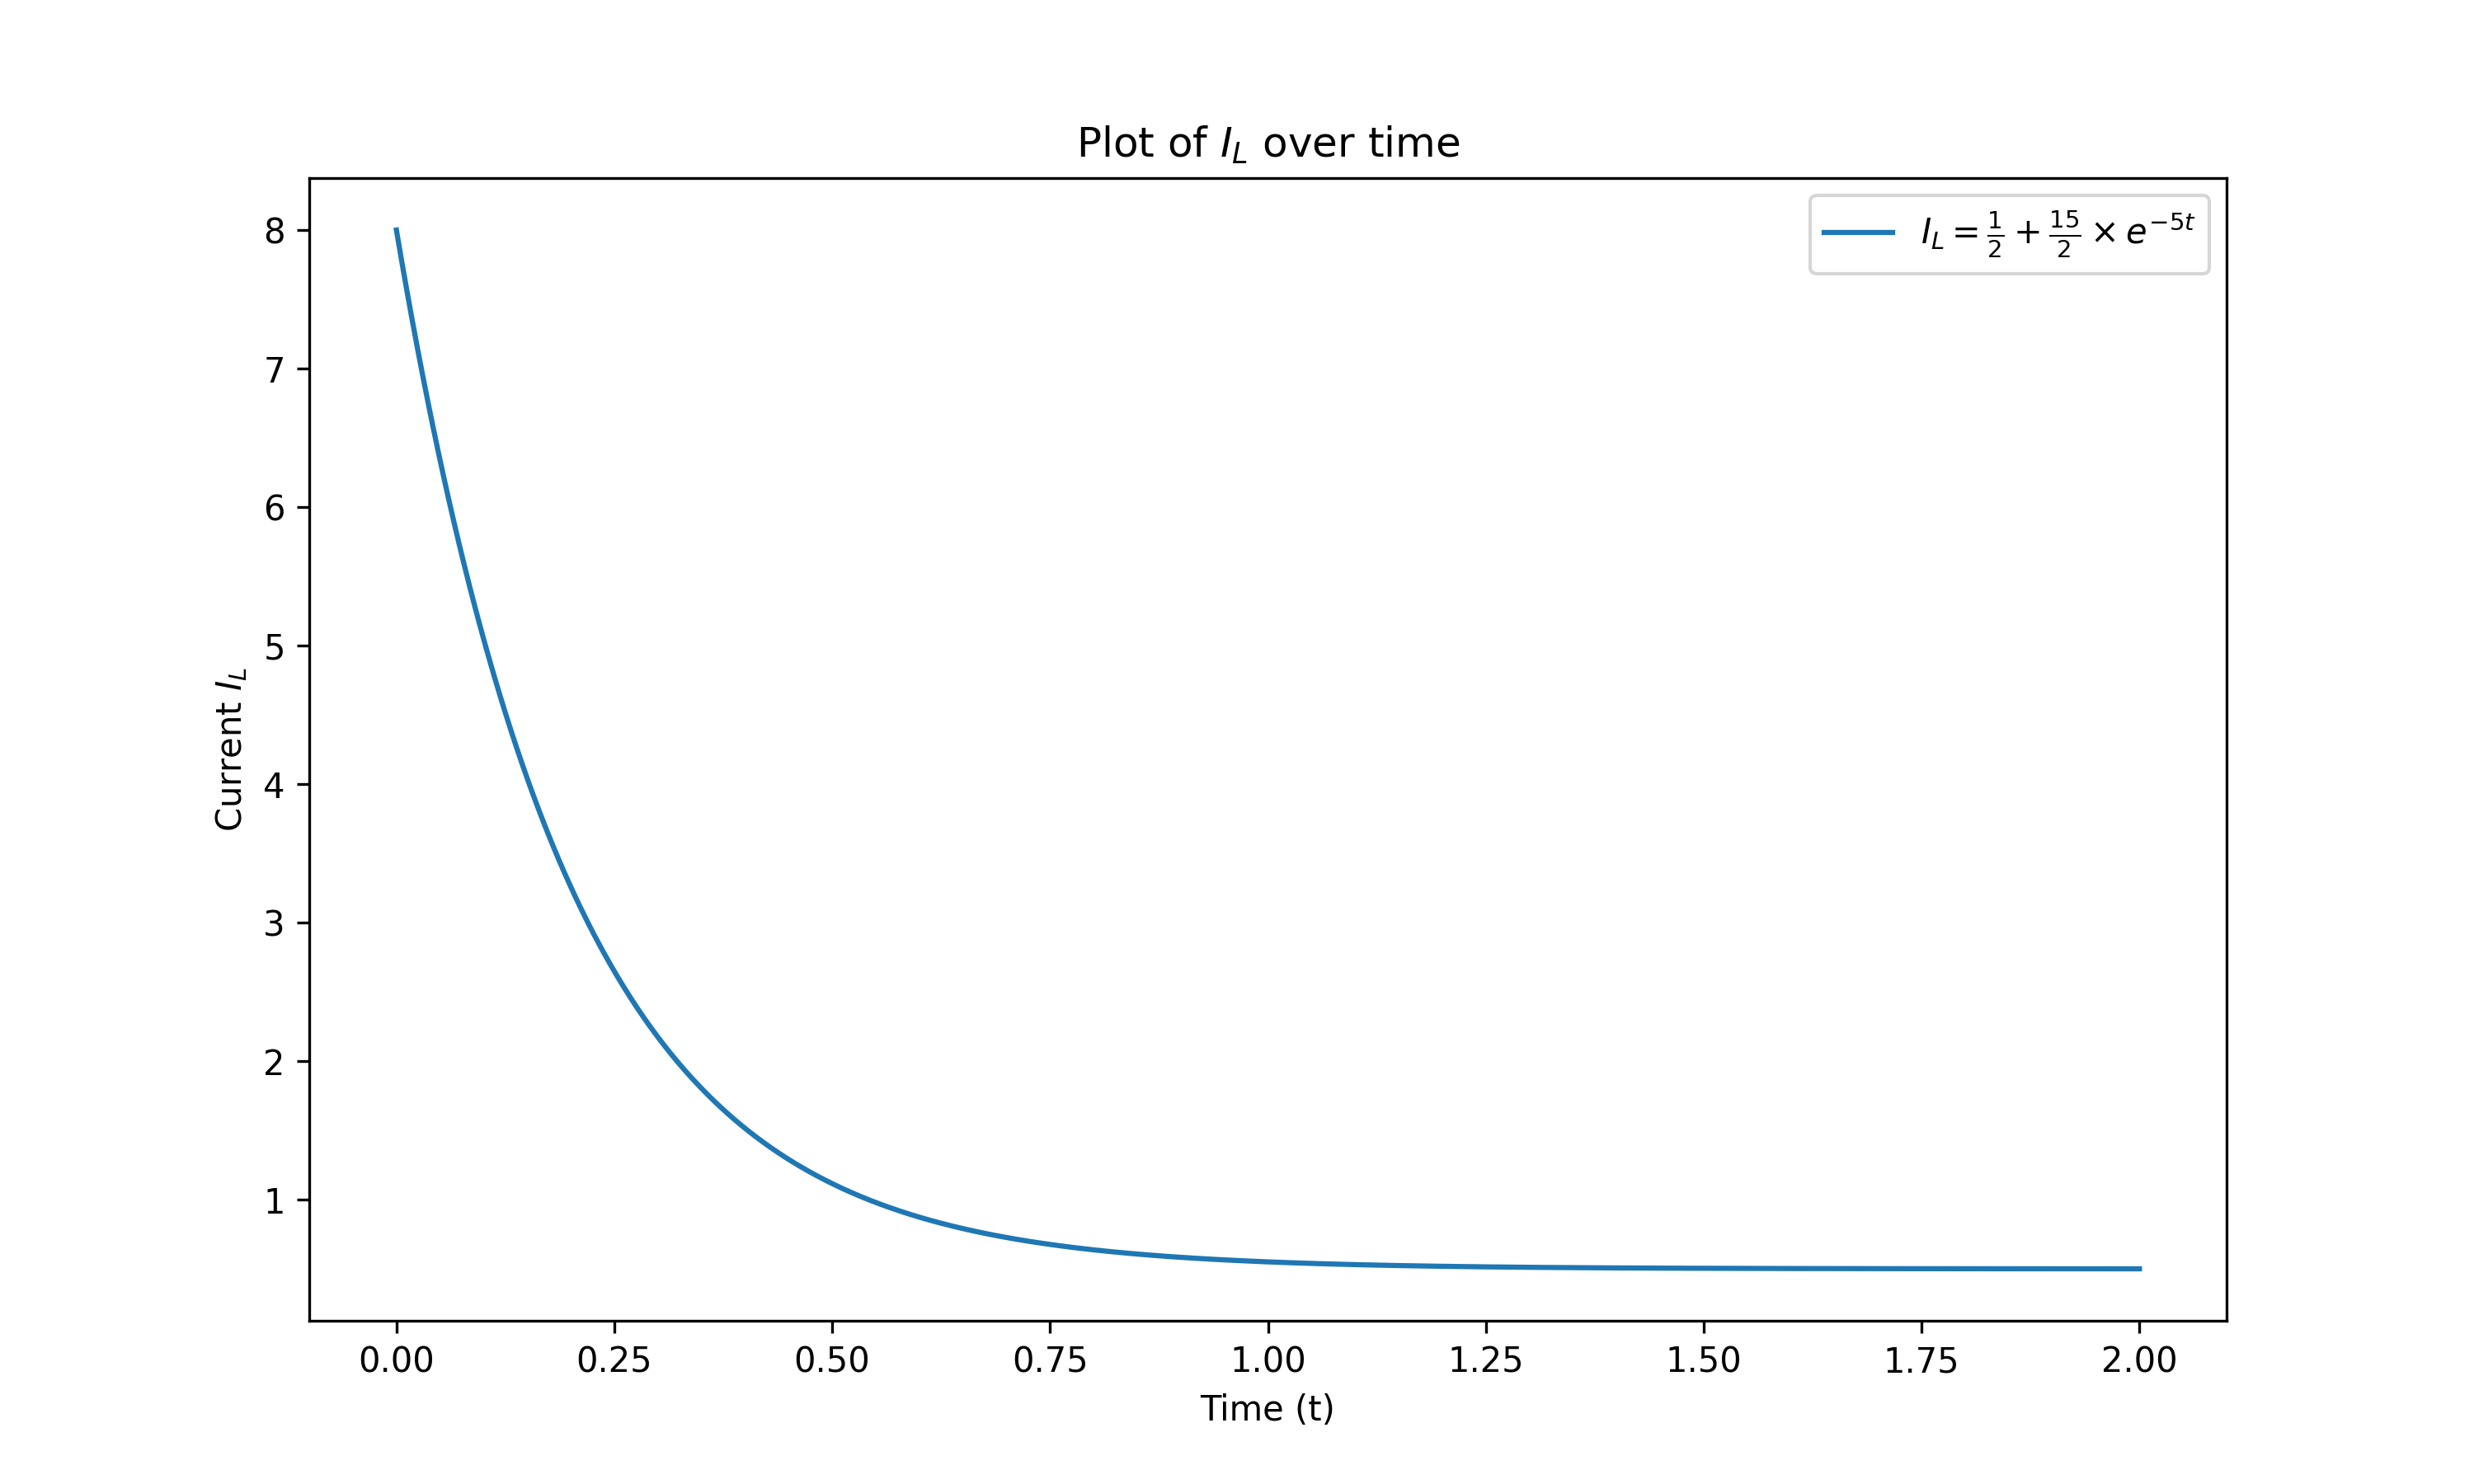
\includegraphics[width=0.9\textwidth, keepaspectratio]{/home/tjoslef/skola/zapisky/vut/IEL/projekt/graf5priklad.png}
  \caption{graf rovnice}
  \label{fig:graf prubehu}
\end{figure}
\end{document}

